\documentclass[12pt, compress, xcolor=table]{beamer}
\usetheme[titleprogressbar]{metropolis}

\usepackage{booktabs}
\usepackage[scale=2]{ccicons}

\usepackage{caption}
\captionsetup[figure]{font=scriptsize,labelfont=scriptsize}
\setlength{\belowcaptionskip}{-10pt}

\title{ARIS - Localization of a Sounding Rocket via GPS}
\author{Simon Herzog}
\institute{Interim Presentation Bachelor Thesis}
\date{April, 2018}

\begin{document}


\maketitle

\begin{frame}{Table of Contents}
 \tableofcontents
\end{frame}


\section{Definition of Task}

\begin{frame}{Framework}
 \begin{columns}
  \column{0.5\textwidth}
  \begin{figure}
  \centering
   
\includegraphics[width=0.9\textwidth]{images/Tell_Logo.png}
  \end{figure}
  \centering{Akademische Raumfahrt Initiative Schweiz}
  
  \column{0.5\textwidth}
  \begin{figure}
   \centering
   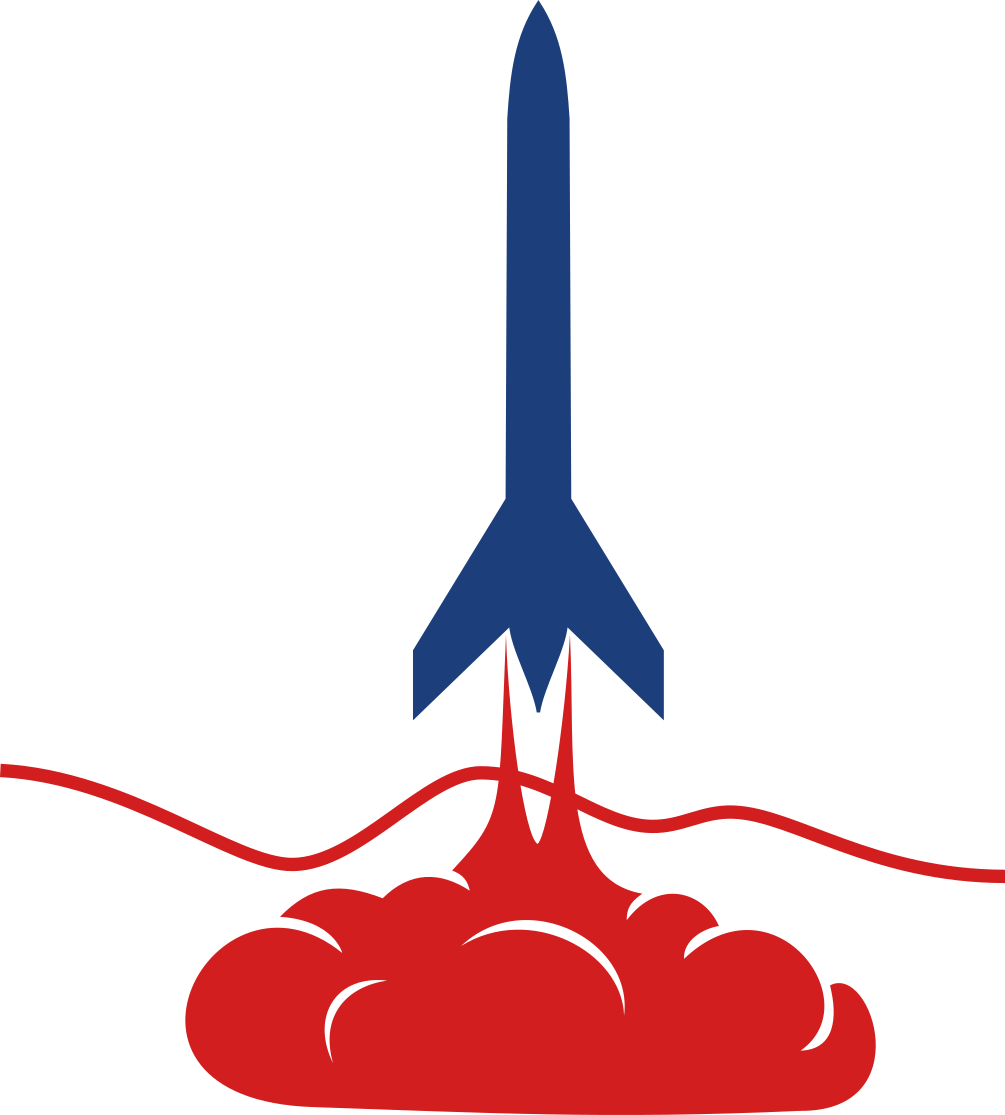
\includegraphics[width=0.9\textwidth]{images/SAC_Logo.png}
   \caption*{Source: spaceportamericacup.com}
  \end{figure}
  \centering{Spaceport America Cup}
  
 \end{columns}
\end{frame}

\begin{frame}{Task}
 \begin{itemize}
  \setlength\itemsep{0.5cm}
  \item Evaluate GPS positioning for a sounding rocket
  \item Determine external and internal disturbances
  \item Find error mitigation methods
  \item Demonstrate feasibility of one method
 \end{itemize}
\end{frame}

\begin{frame}{Requirements}
 \begin{itemize}
  \setlength\itemsep{0.5cm}
  \item Positioning Standard Deviation($1\sigma$): 1m \\[30pt]
  \item Min. Update Interval: 60s
  \item Max. TTFF after Burnout: 2s
  \item Max. Uplink Datarate: 2kbit/s
 \end{itemize}
\end{frame}


\section{GPS Concept}

\begin{frame}{GPS Overview}
  \begin{columns}
    \column{0.5\textwidth}

    \begin{itemize}
    
      \item Space Segment
      \begin{tabbing}
      \hspace*{0.5cm}\= \kill
      \> \footnotesize{31 Satellites (min. 24) in} \\
      \> \footnotesize{Medium Earth Orbit} \\
      \end{tabbing}

      \item Control Segment
      \begin{tabbing}
      \hspace*{0.5cm}\= \kill
      \> \footnotesize{Monitorung and Maintanance} \\
      \> \footnotesize{Stations} \\
      \end{tabbing}
      
      \item User Segment
      \begin{tabbing}
      \hspace*{0.5cm}\= \kill
      \> \footnotesize{Civil and Military Receivers}
      \end{tabbing}
      
    \end{itemize}
 
    \column{0.5\textwidth}
    \begin{figure}
     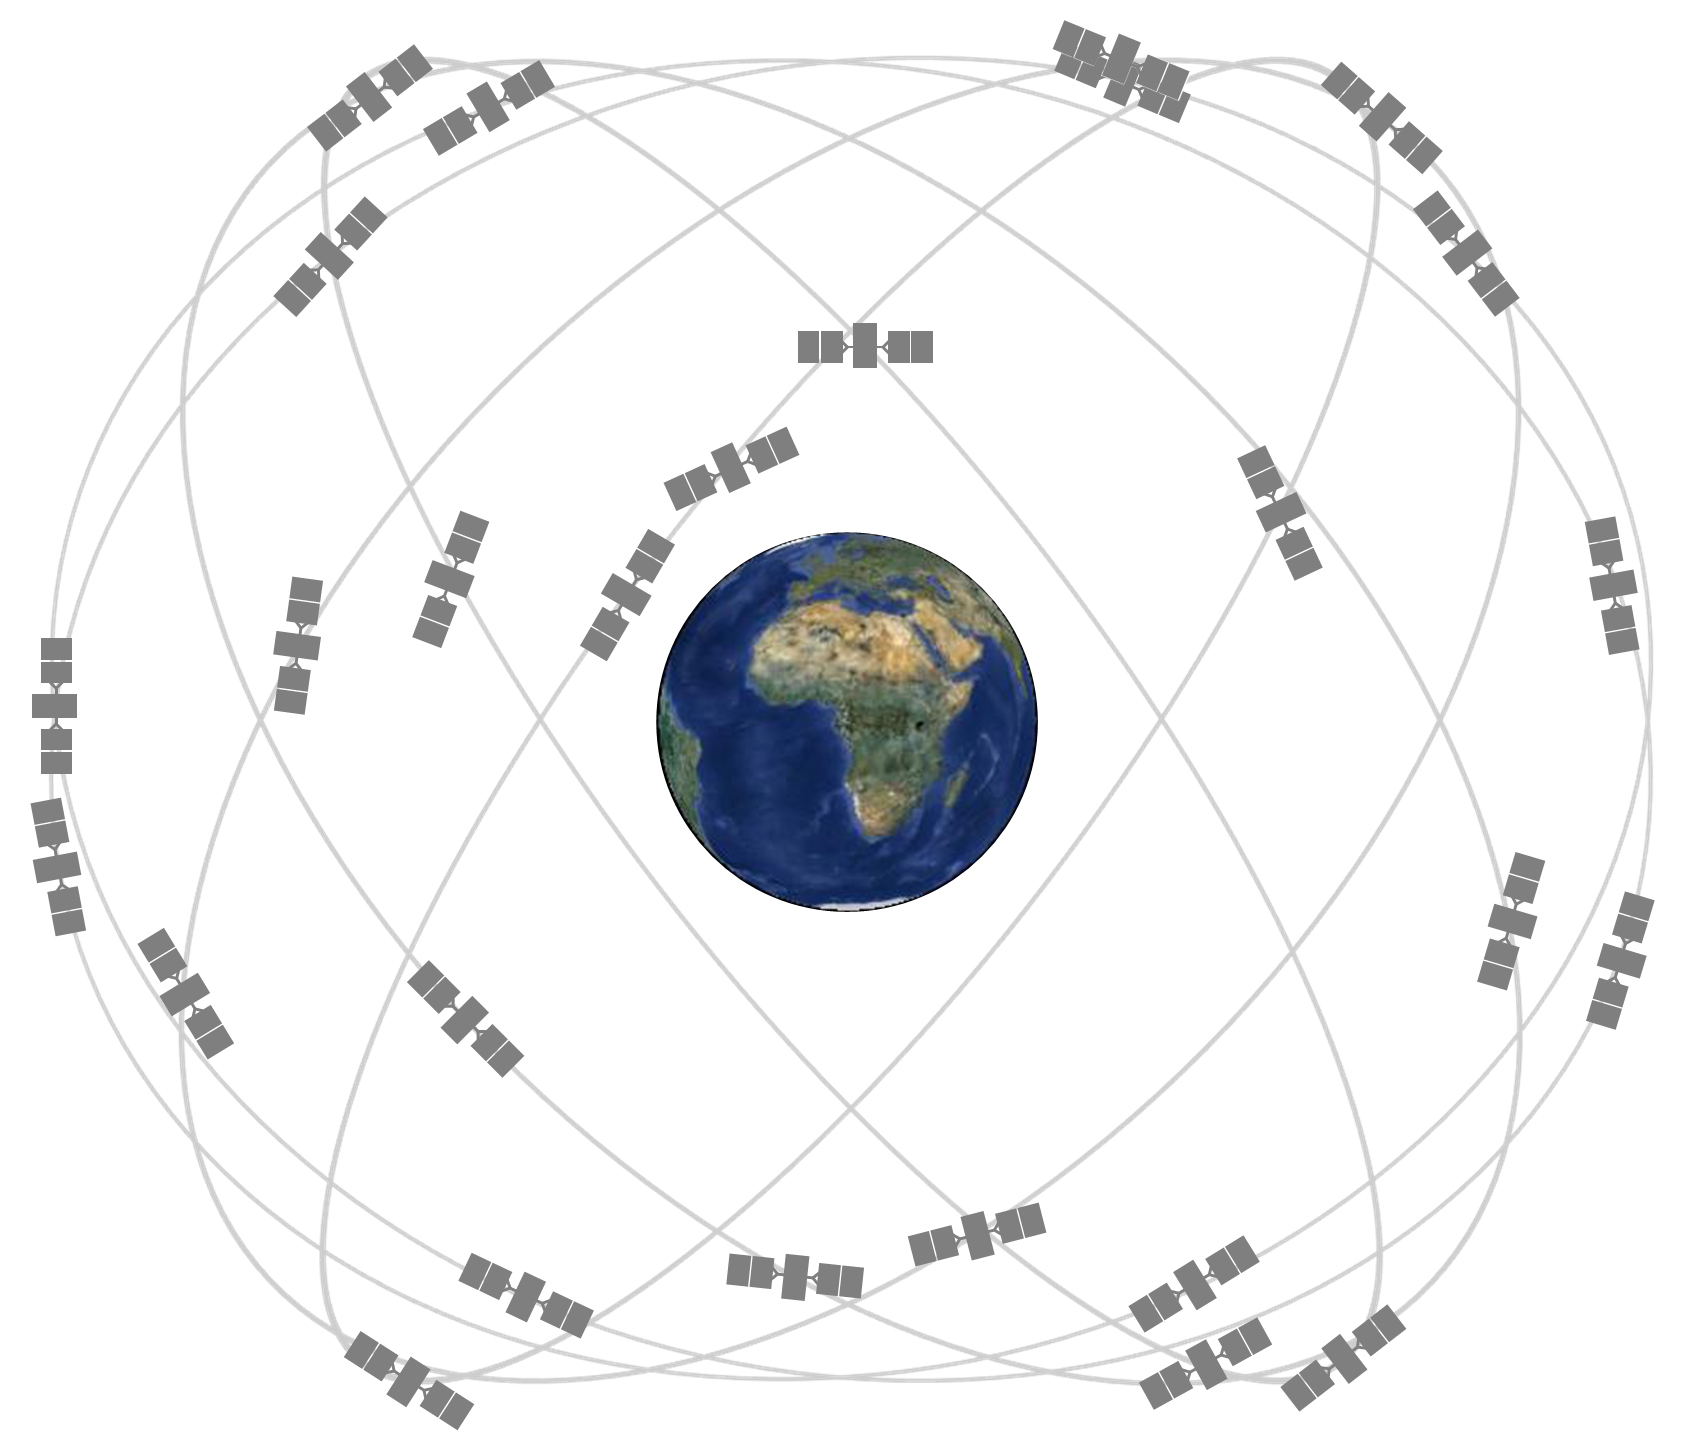
\includegraphics[width=\textwidth]{images/constellation.jpg}
    \caption*{Source: gps.gov}
    \end{figure}
  \end{columns}
\end{frame}

\begin{frame}{Position Estimation}
 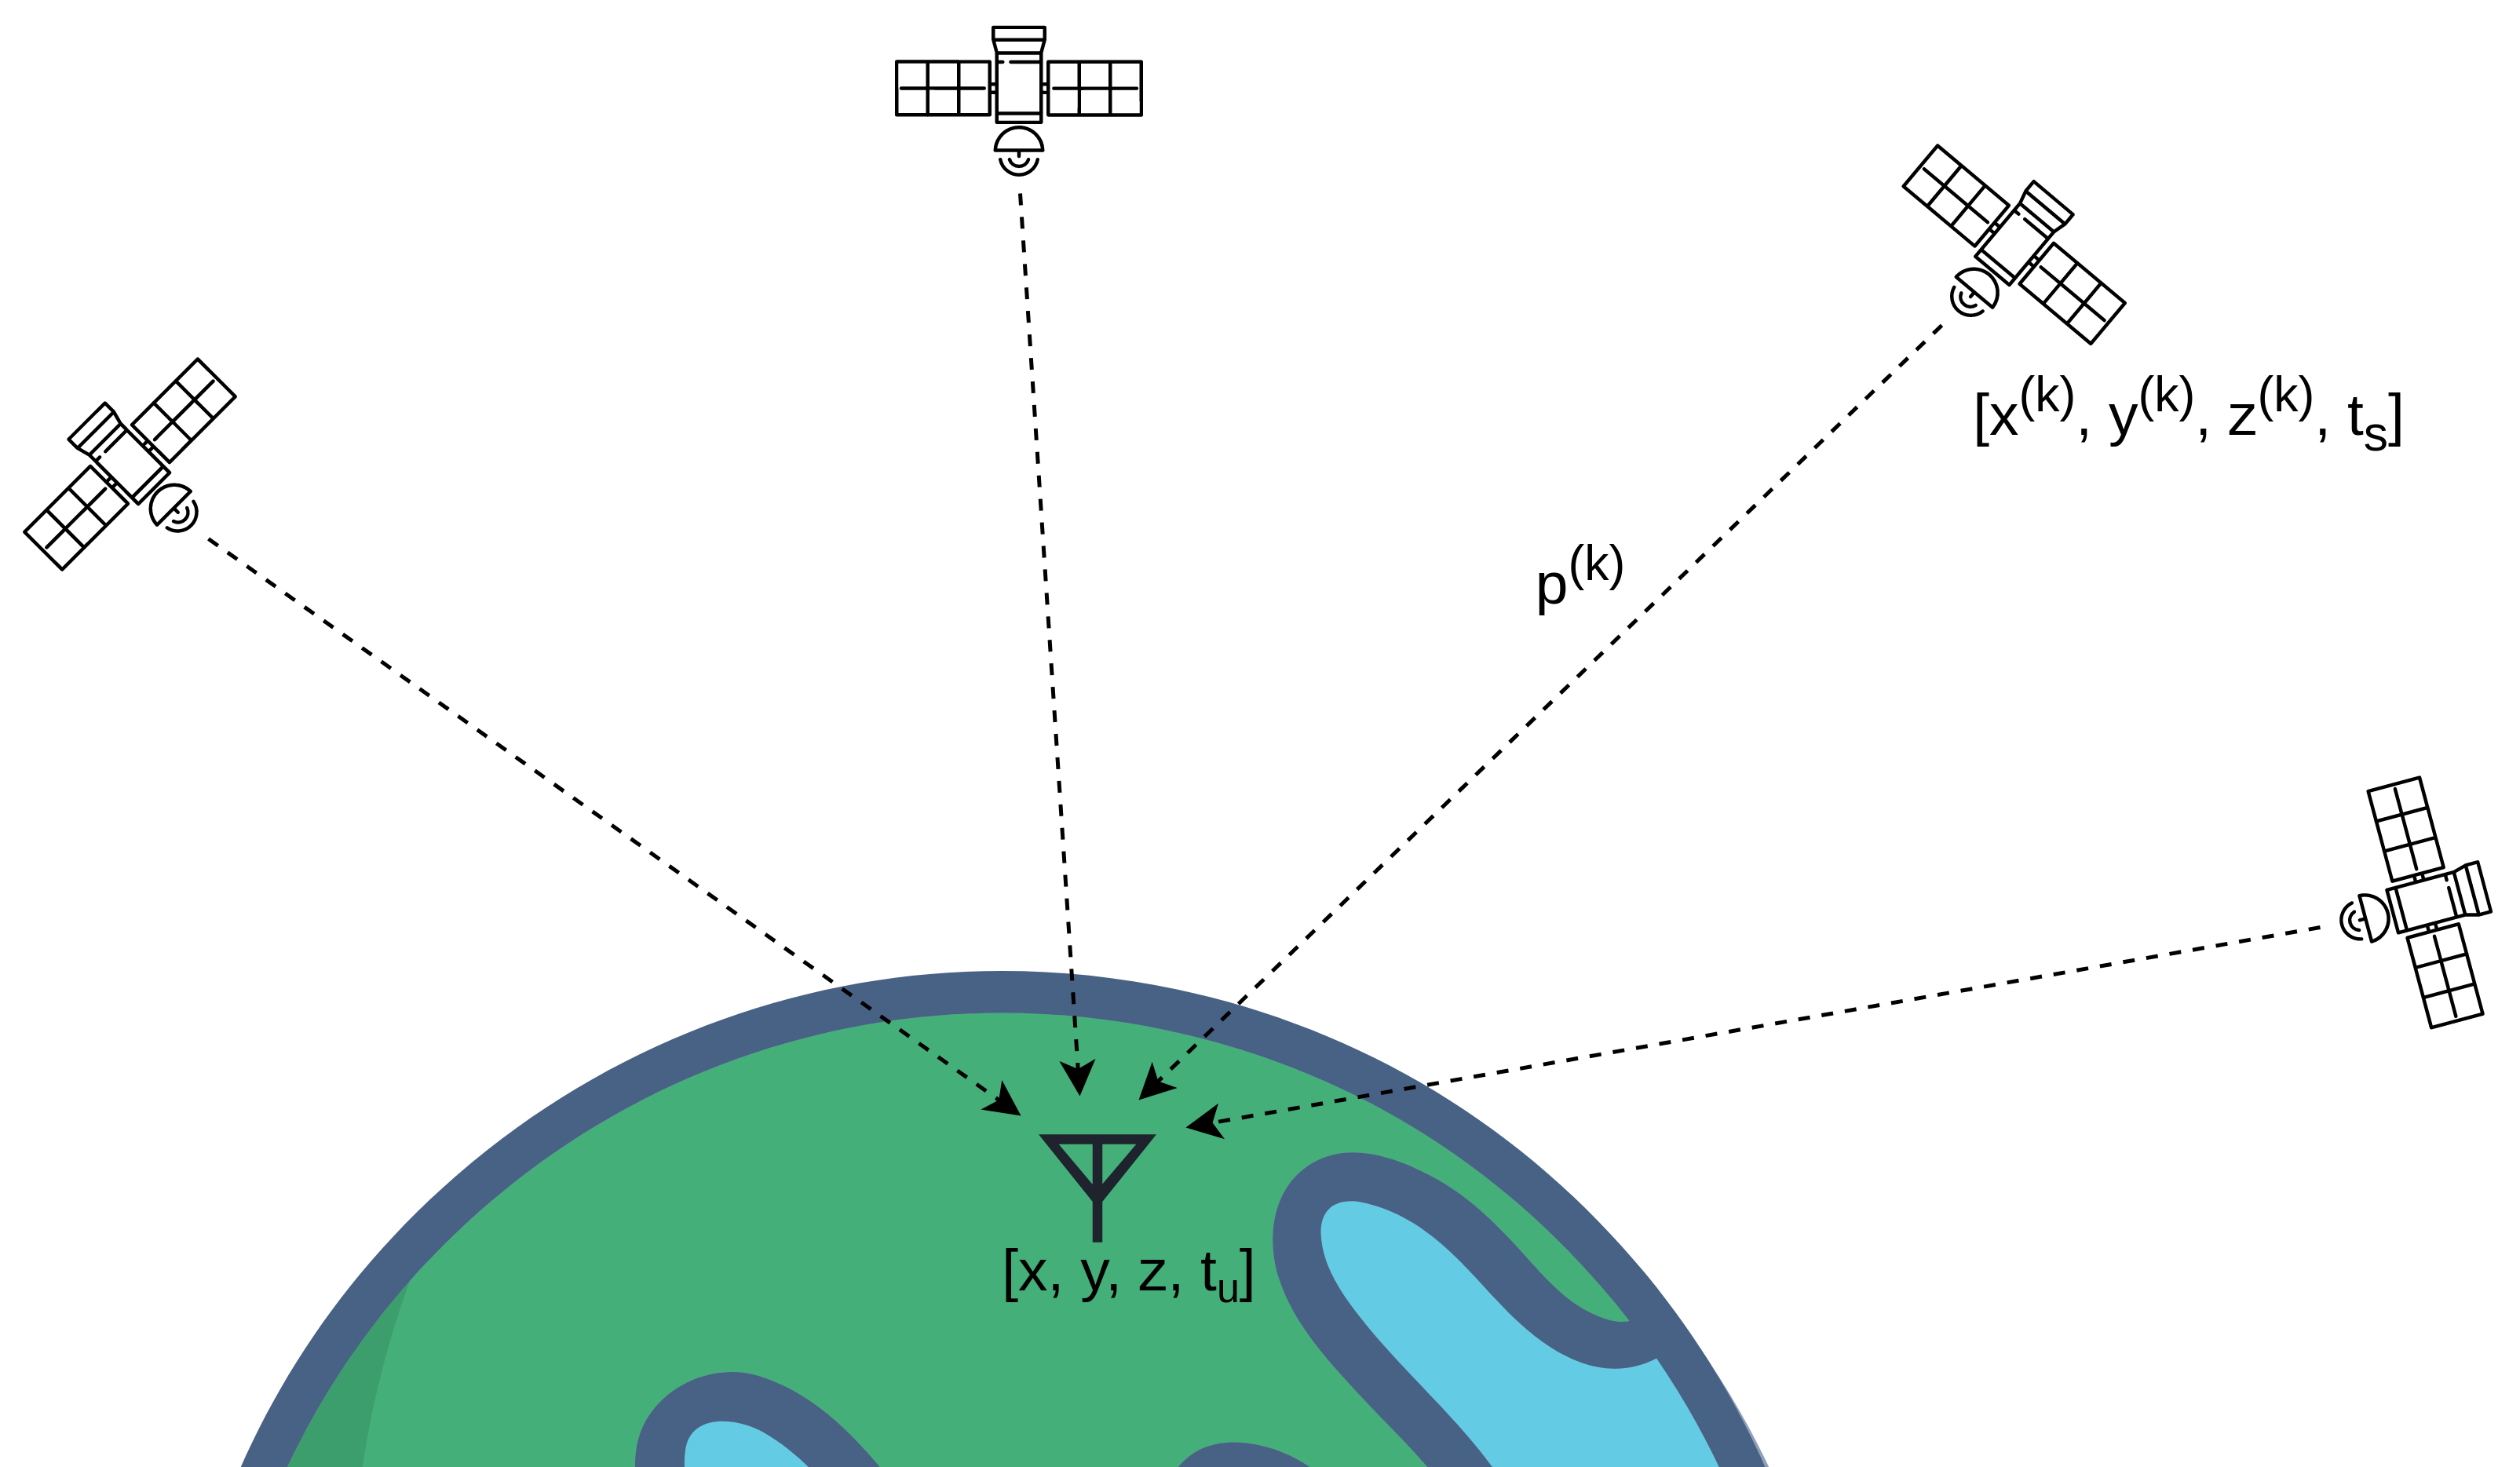
\includegraphics[width=\textwidth]{images/Position_Estimation.png}
\end{frame}


\section{Errors Sources}

\begin{frame}{Satellite Errors}
 \begin{columns}
  \column{0.5\textwidth}
  \begin{itemize}
  \setlength\itemsep{0.5cm}
   \item Clock Error
   \item Ephemeris Error
  \end{itemize}

  \column{0.5\textwidth}
  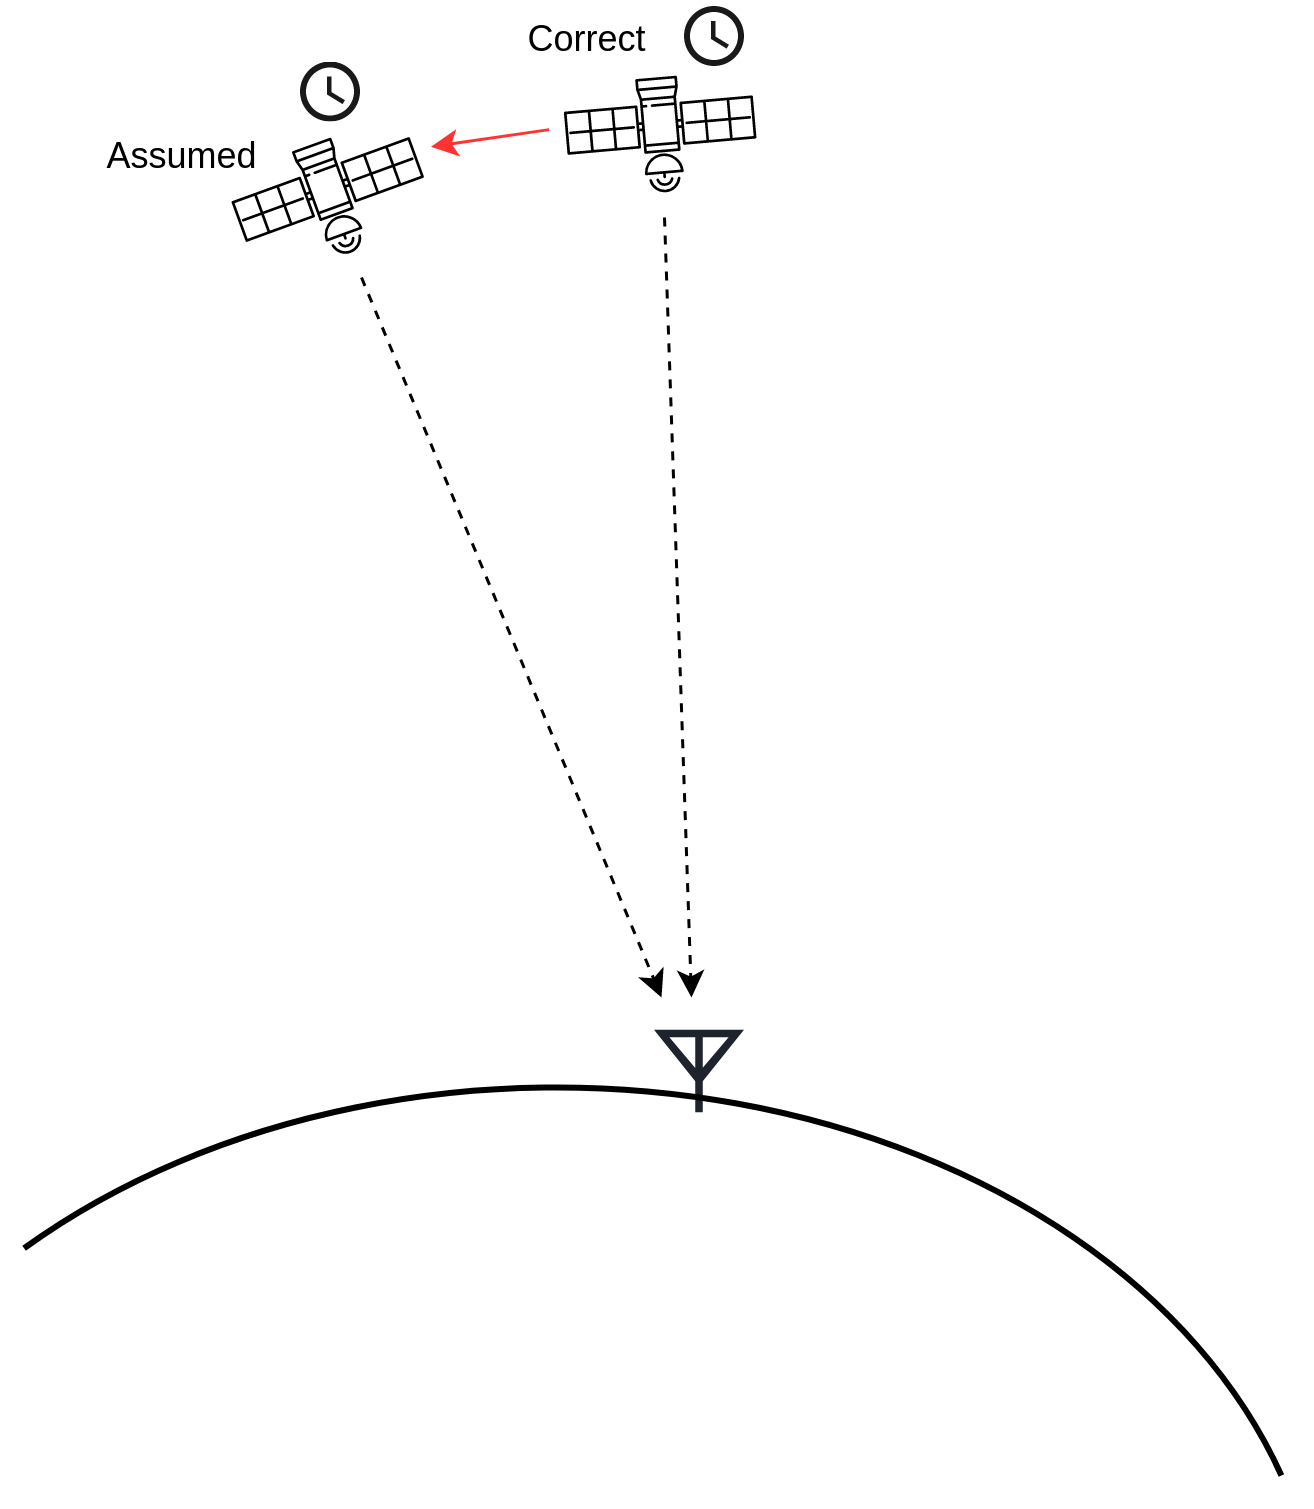
\includegraphics[width=\textwidth]{images/Satellite_Error.png}
  
 \end{columns}
\end{frame}

\begin{frame}{Atmospheric Errors}
 \begin{columns}
  \column{0.5\textwidth}
  \begin{itemize}
  \setlength\itemsep{0.5cm}
   \item Ionospheric Delay
   \item Tropospheric Delay
  \end{itemize}

  \column{0.5\textwidth}
  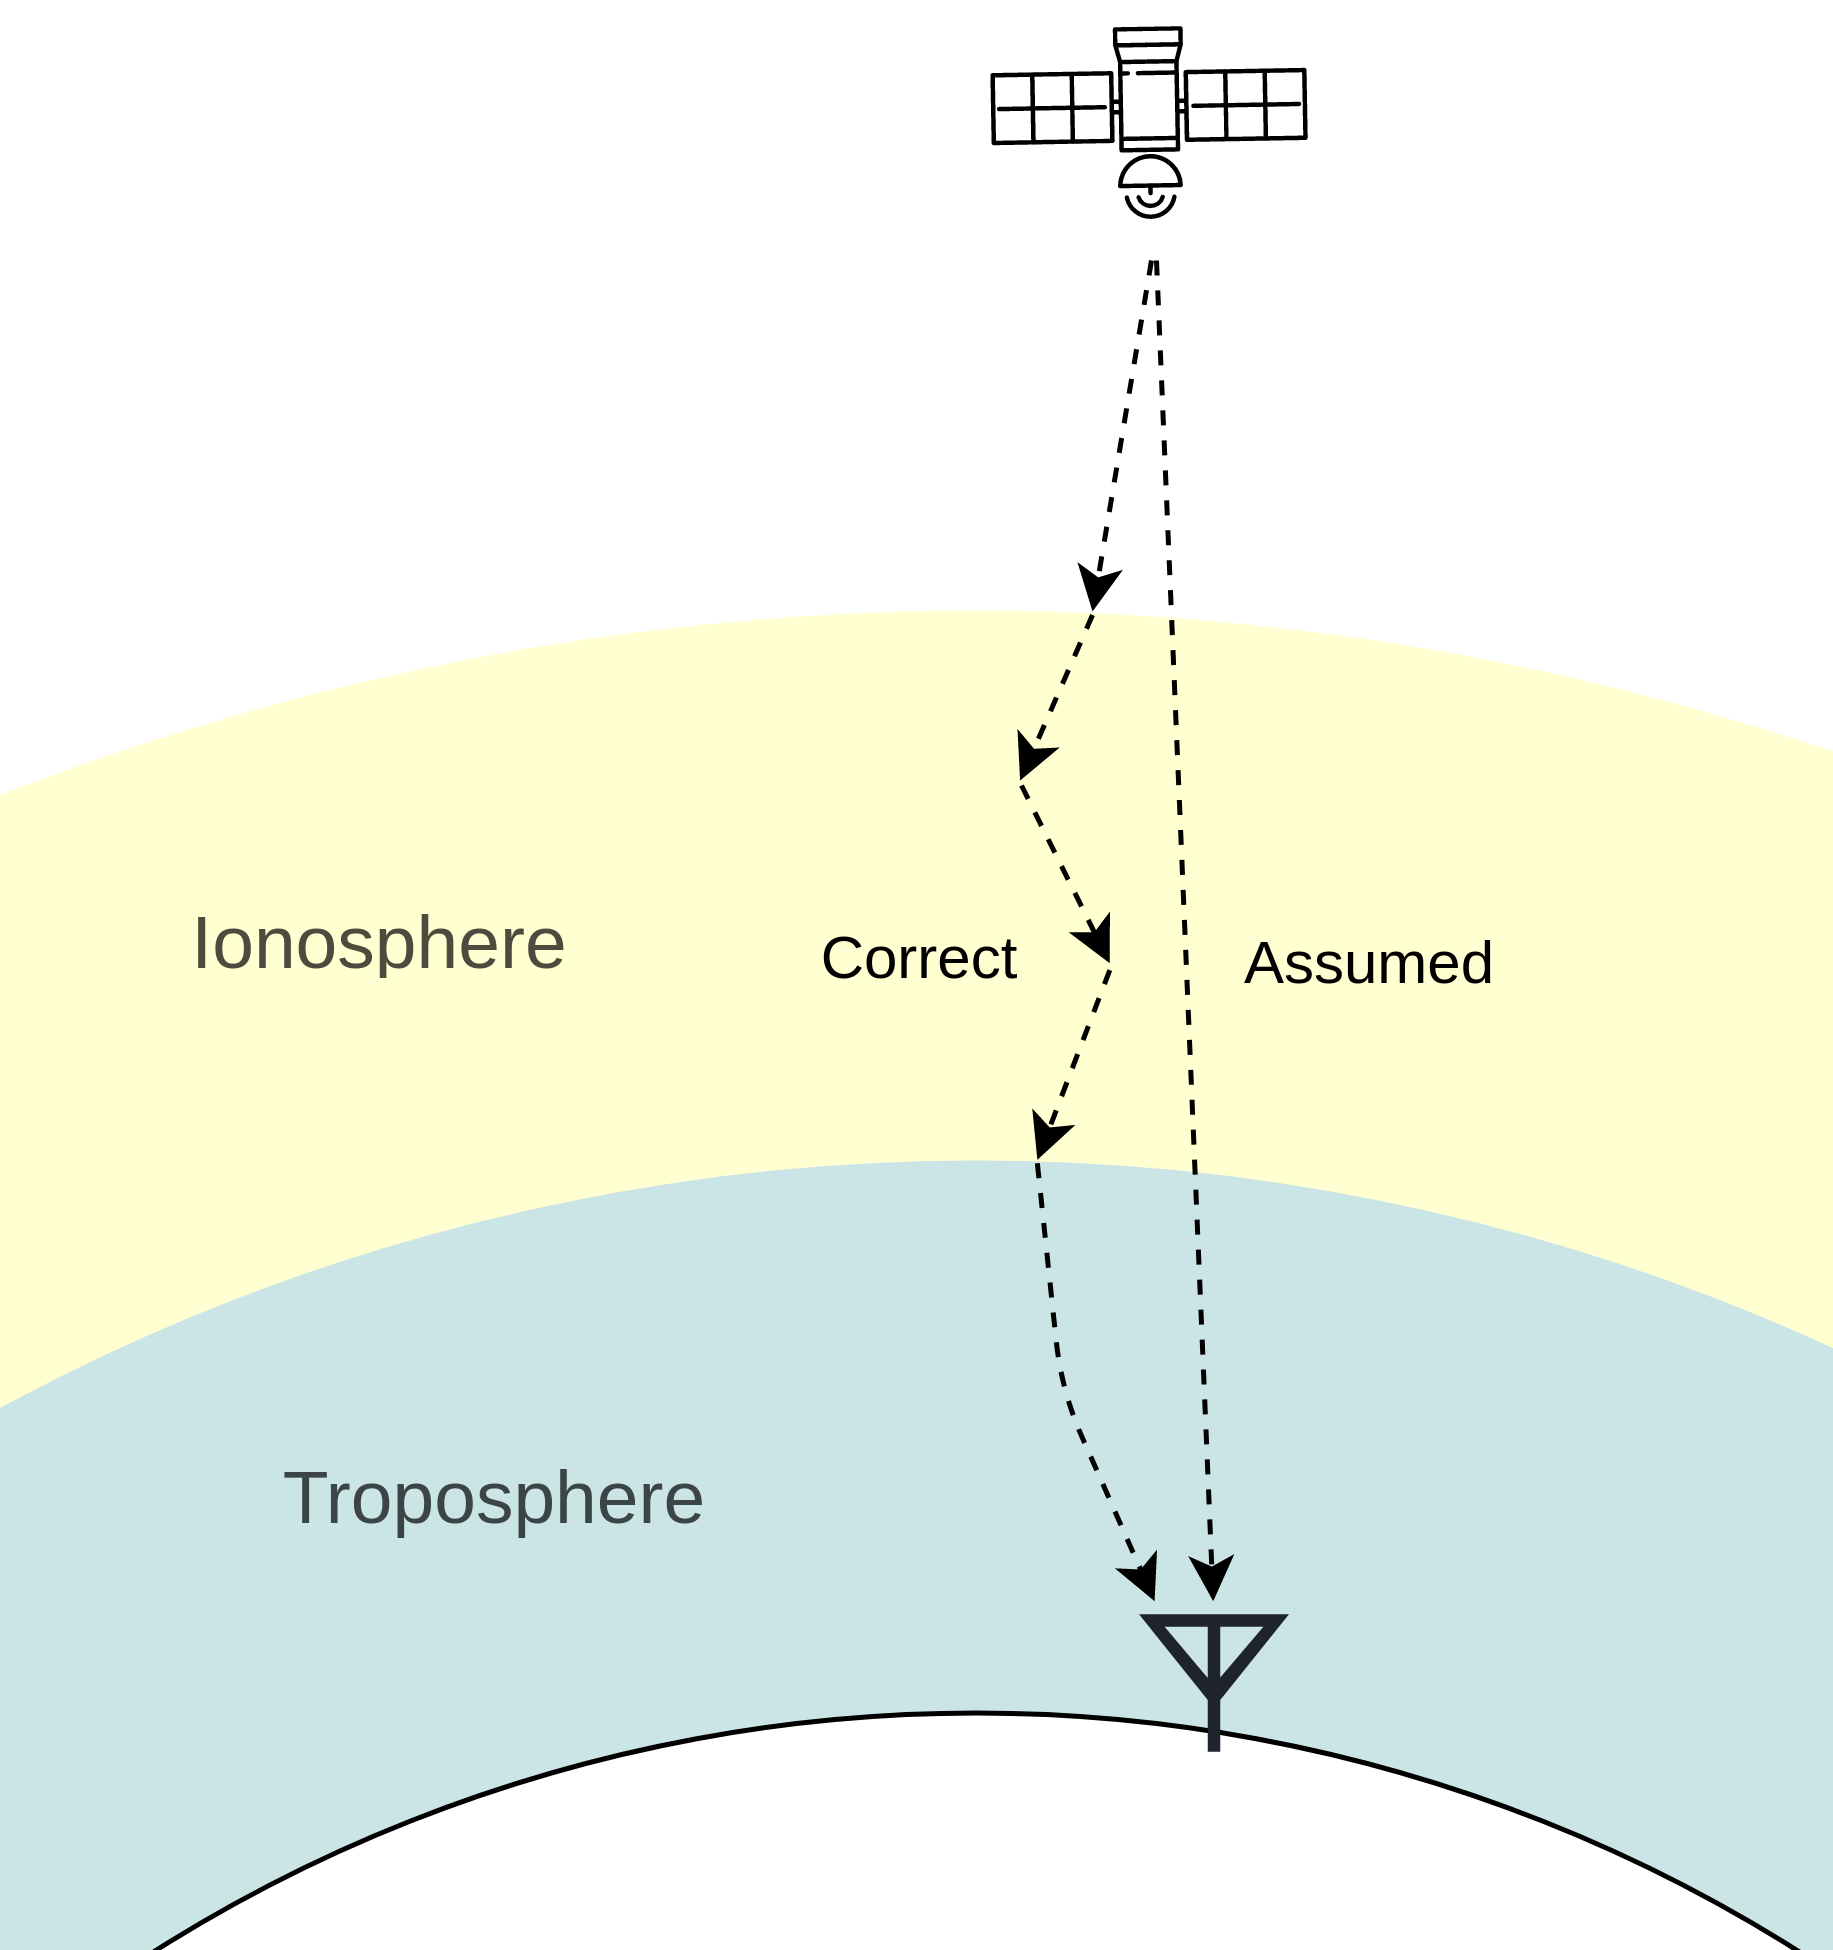
\includegraphics[width=\textwidth]{images/Atmospheric_Error.png}
  
 \end{columns}
\end{frame}

\begin{frame}{Receiver Errors}
 \begin{columns}
  \column{0.5\textwidth}
  \begin{itemize}
  \setlength\itemsep{0.5cm}
   \item Multipath
   \item Receiver Noise
  \end{itemize}

  \column{0.5\textwidth}
  
\includegraphics[width=\textwidth]{images/Multipath.png}
  
  \hspace{1cm}
  
  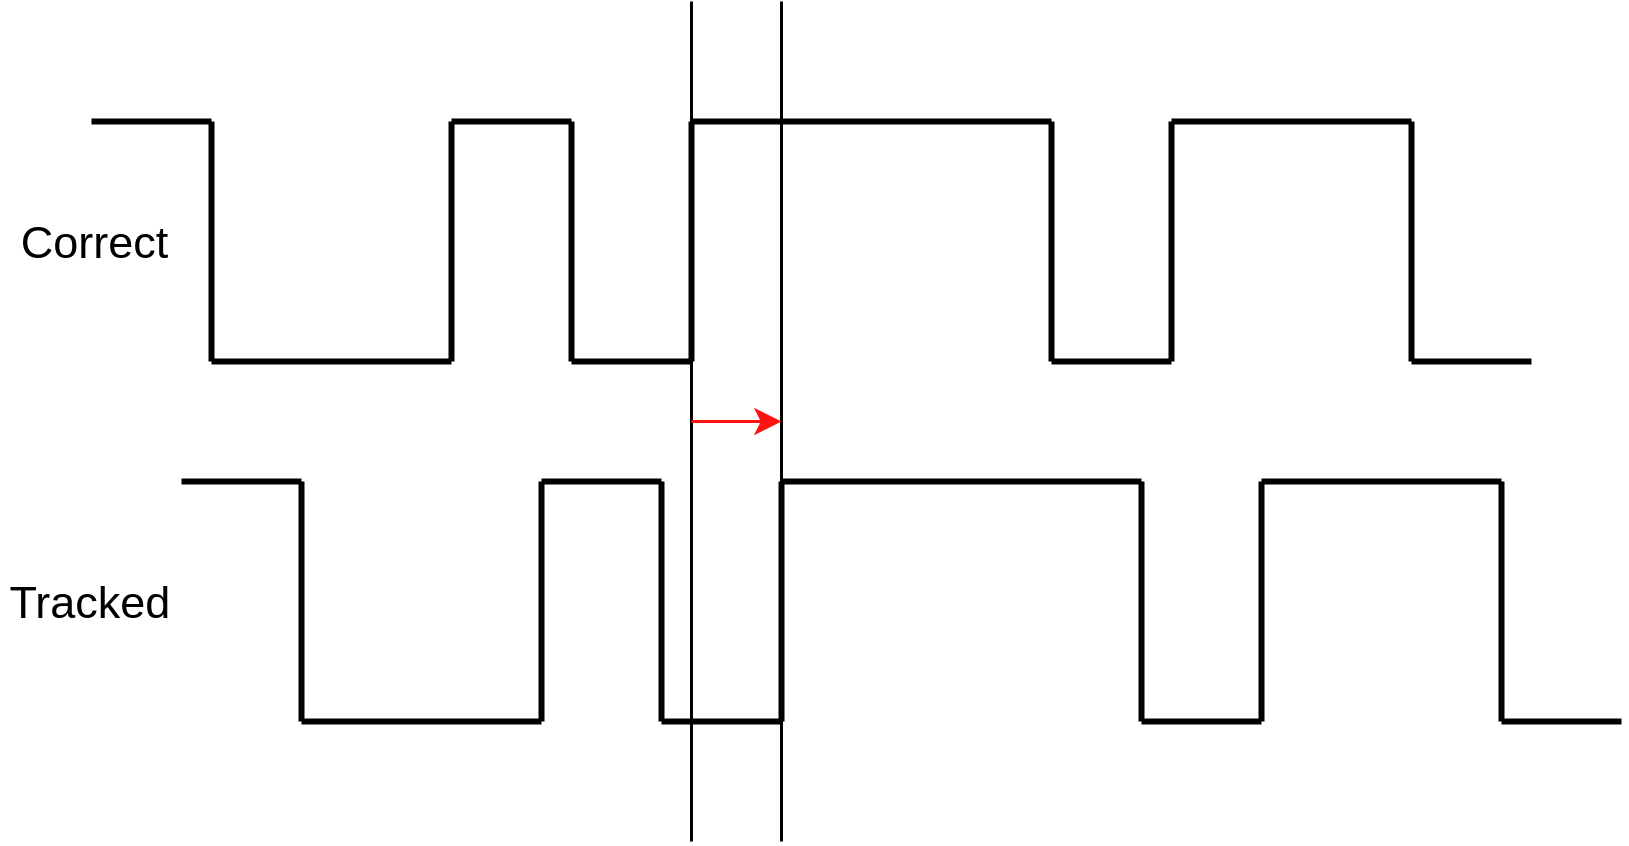
\includegraphics[width=\textwidth]{images/Receiver_Noise.png}
  
 \end{columns}
\end{frame}

\begin{frame}{Error Mitigation}
  \begin{columns}
  \column{0.5\textwidth}
  \begin{itemize}
  \setlength\itemsep{0.5cm}
   \item Carrier-Phase Measurements
   \item Differential GPS
   \item Real Time Kinematic
  \end{itemize}

  \column{0.5\textwidth}
  \begin{figure}
   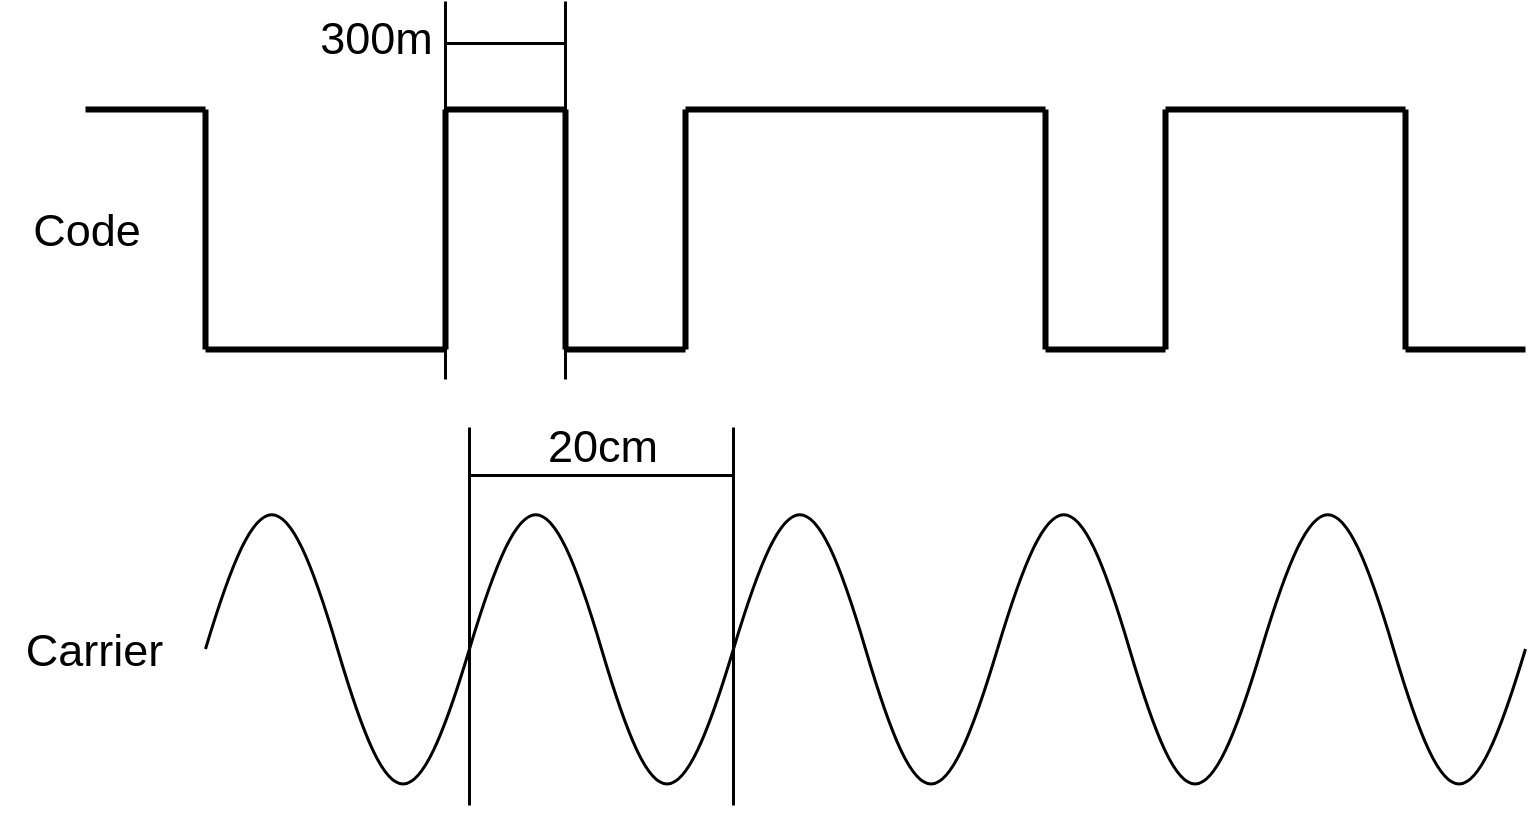
\includegraphics[height=0.3\textheight]{images/Carrier-Phase_Measurement.png}
  
  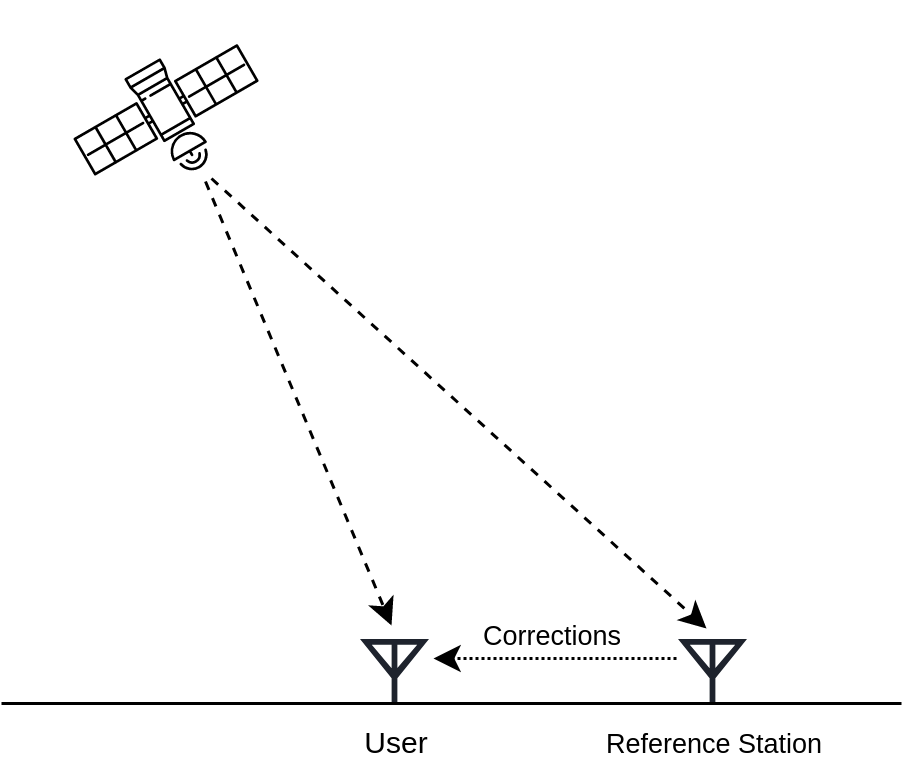
\includegraphics[height=0.45\textheight]{images/Differential_GPS.png}
  \end{figure}   
  
 \end{columns}
\end{frame}


\section{DGPS Concept for a Sounding Rocket}

\begin{frame}{Concept}
 \begin{columns}
  \column{0.5\textwidth}
  \begin{itemize}
   \footnotesize
   \item Position of RS is known
   \item RS receives satellite epehemeris data
   \item Pseudorange between RS and satellite is measured
   \item Distance between RS and satellite is calculated
   \item Range error of every visible satellite is sent to rocket
   \item Receiver on rocket includes corrections in position estimation
  \end{itemize}

  \column{0.5\textwidth}
  \begin{figure}
   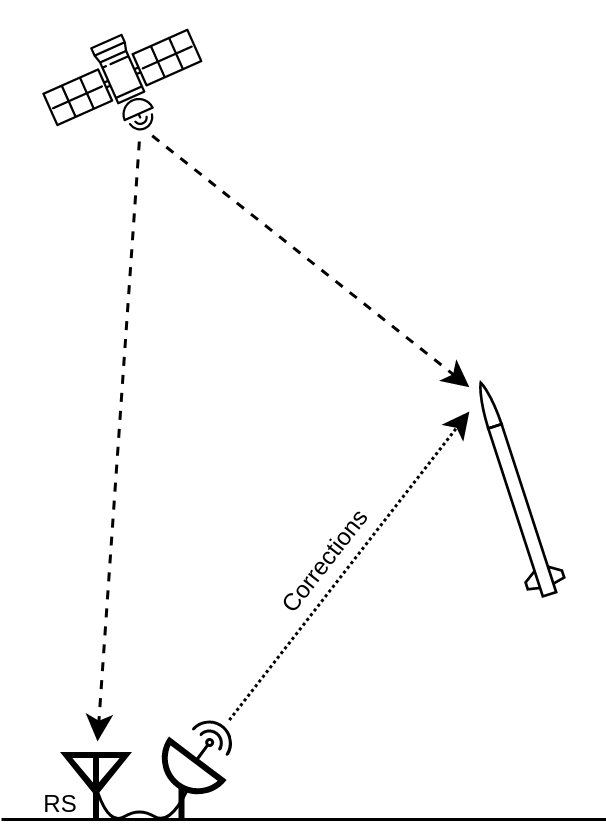
\includegraphics[width=\textwidth]{images/DGPS_Rocket_Concept.png}
  \end{figure}   
  
 \end{columns}
\end{frame}

\begin{frame}{System Overview}
 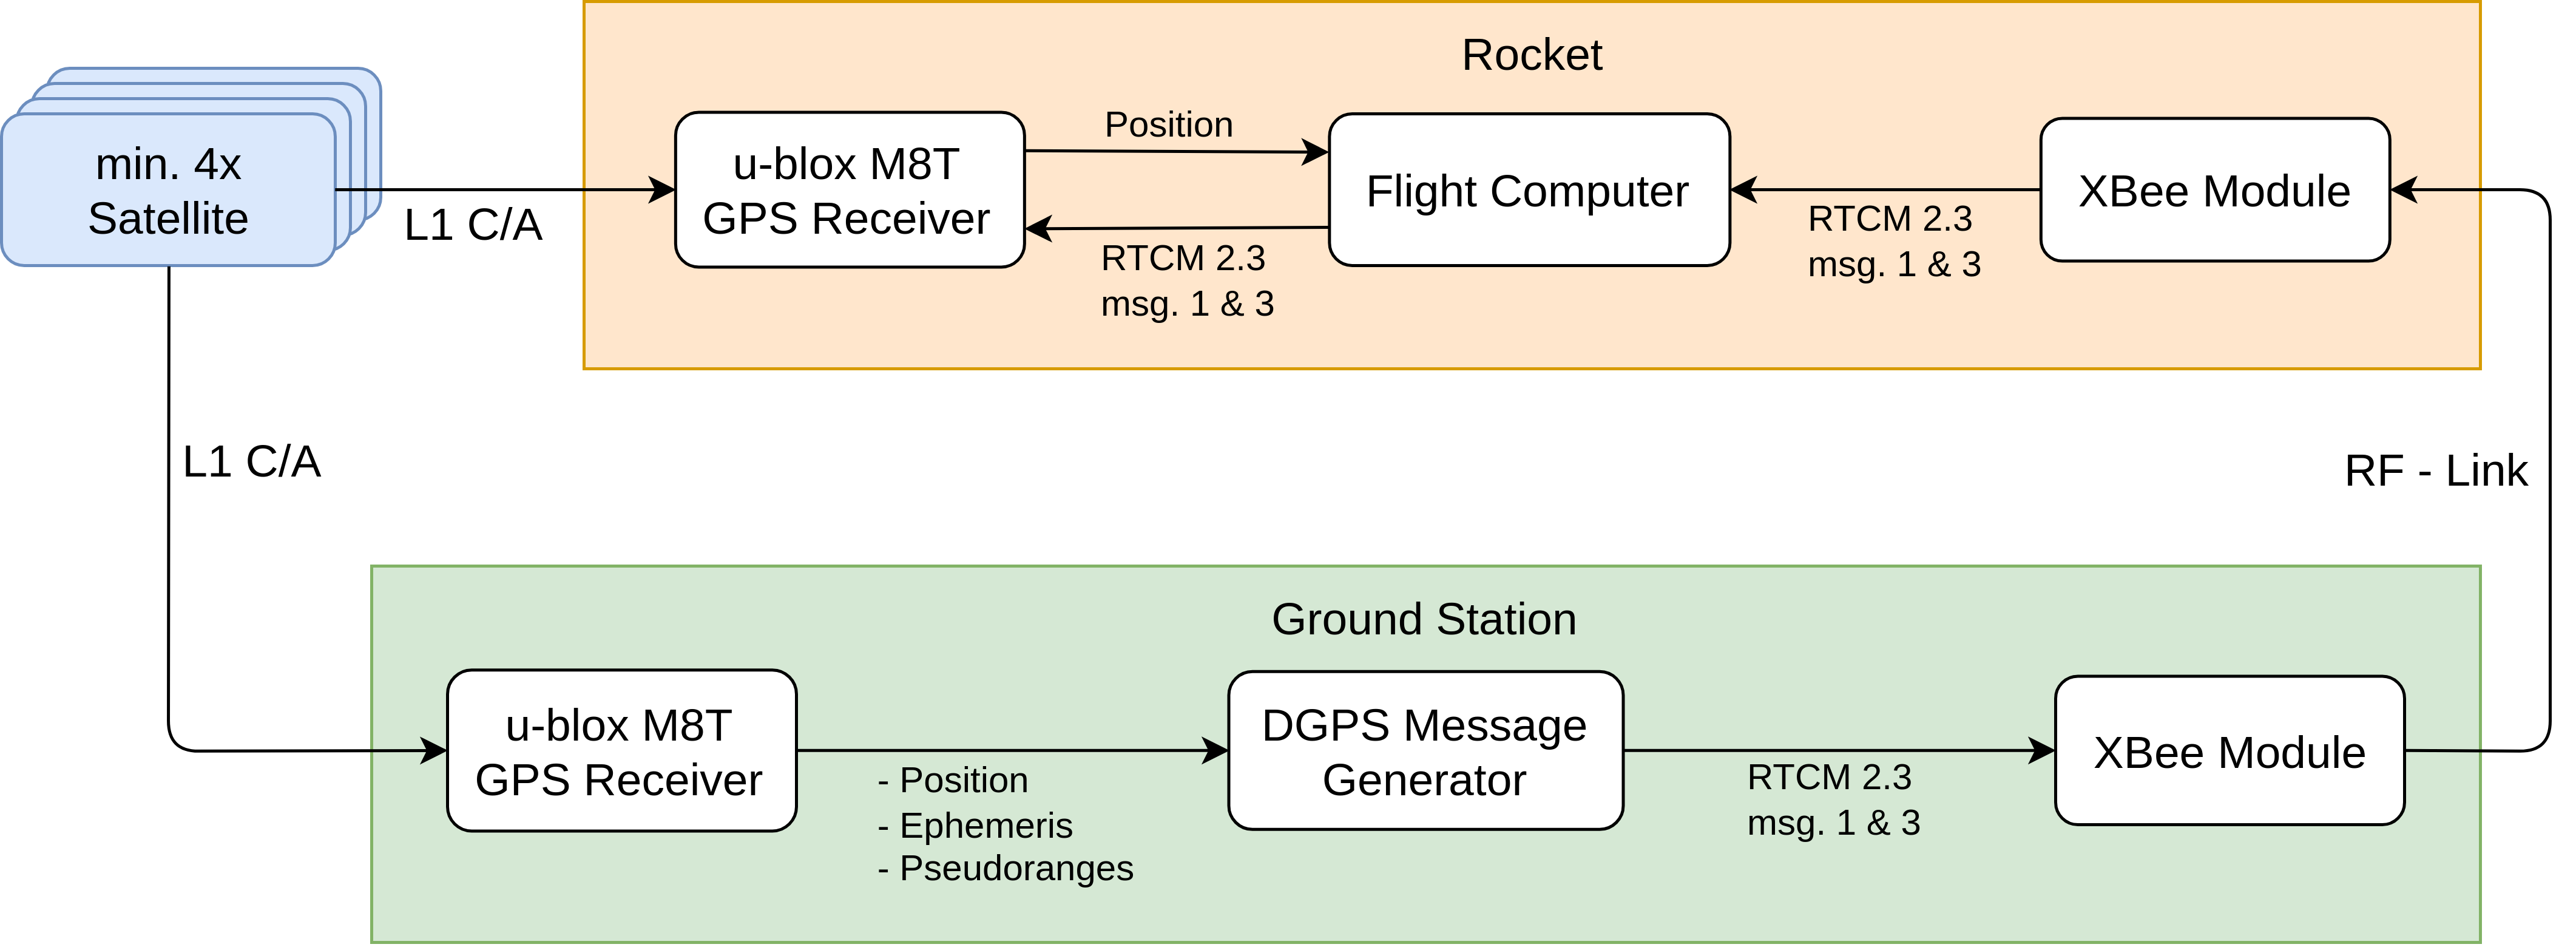
\includegraphics[width=\textwidth]{images/DGPS_System_Overview.png}
\end{frame}

\begin{frame}{DGPS Message Generator}
 \begin{columns}
  \column{0.6\textwidth}
  \begin{itemize}
   \setlength\itemsep{0.3cm}
   \item Receive UBX messages
   \item Set reference positon
   \item Decode ephemeris data
   \item Calculate satellite position
   \item Calculate pseudorange error
   \item Encode RTCM messages
   \item Send RTCM messages
  \end{itemize}
  
  \column{0.35\textwidth}
  \begin{figure}
   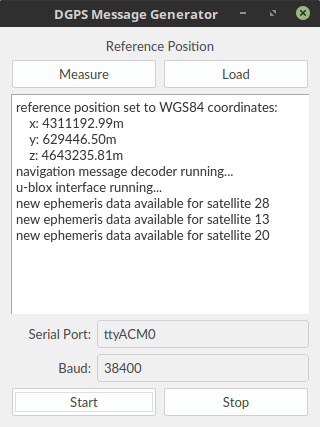
\includegraphics[width=\textwidth]{images/DGPS_Message_Generator_GUI.png}
  \end{figure}
  
 \end{columns}
\end{frame}

\begin{frame}{Software Architecture}
 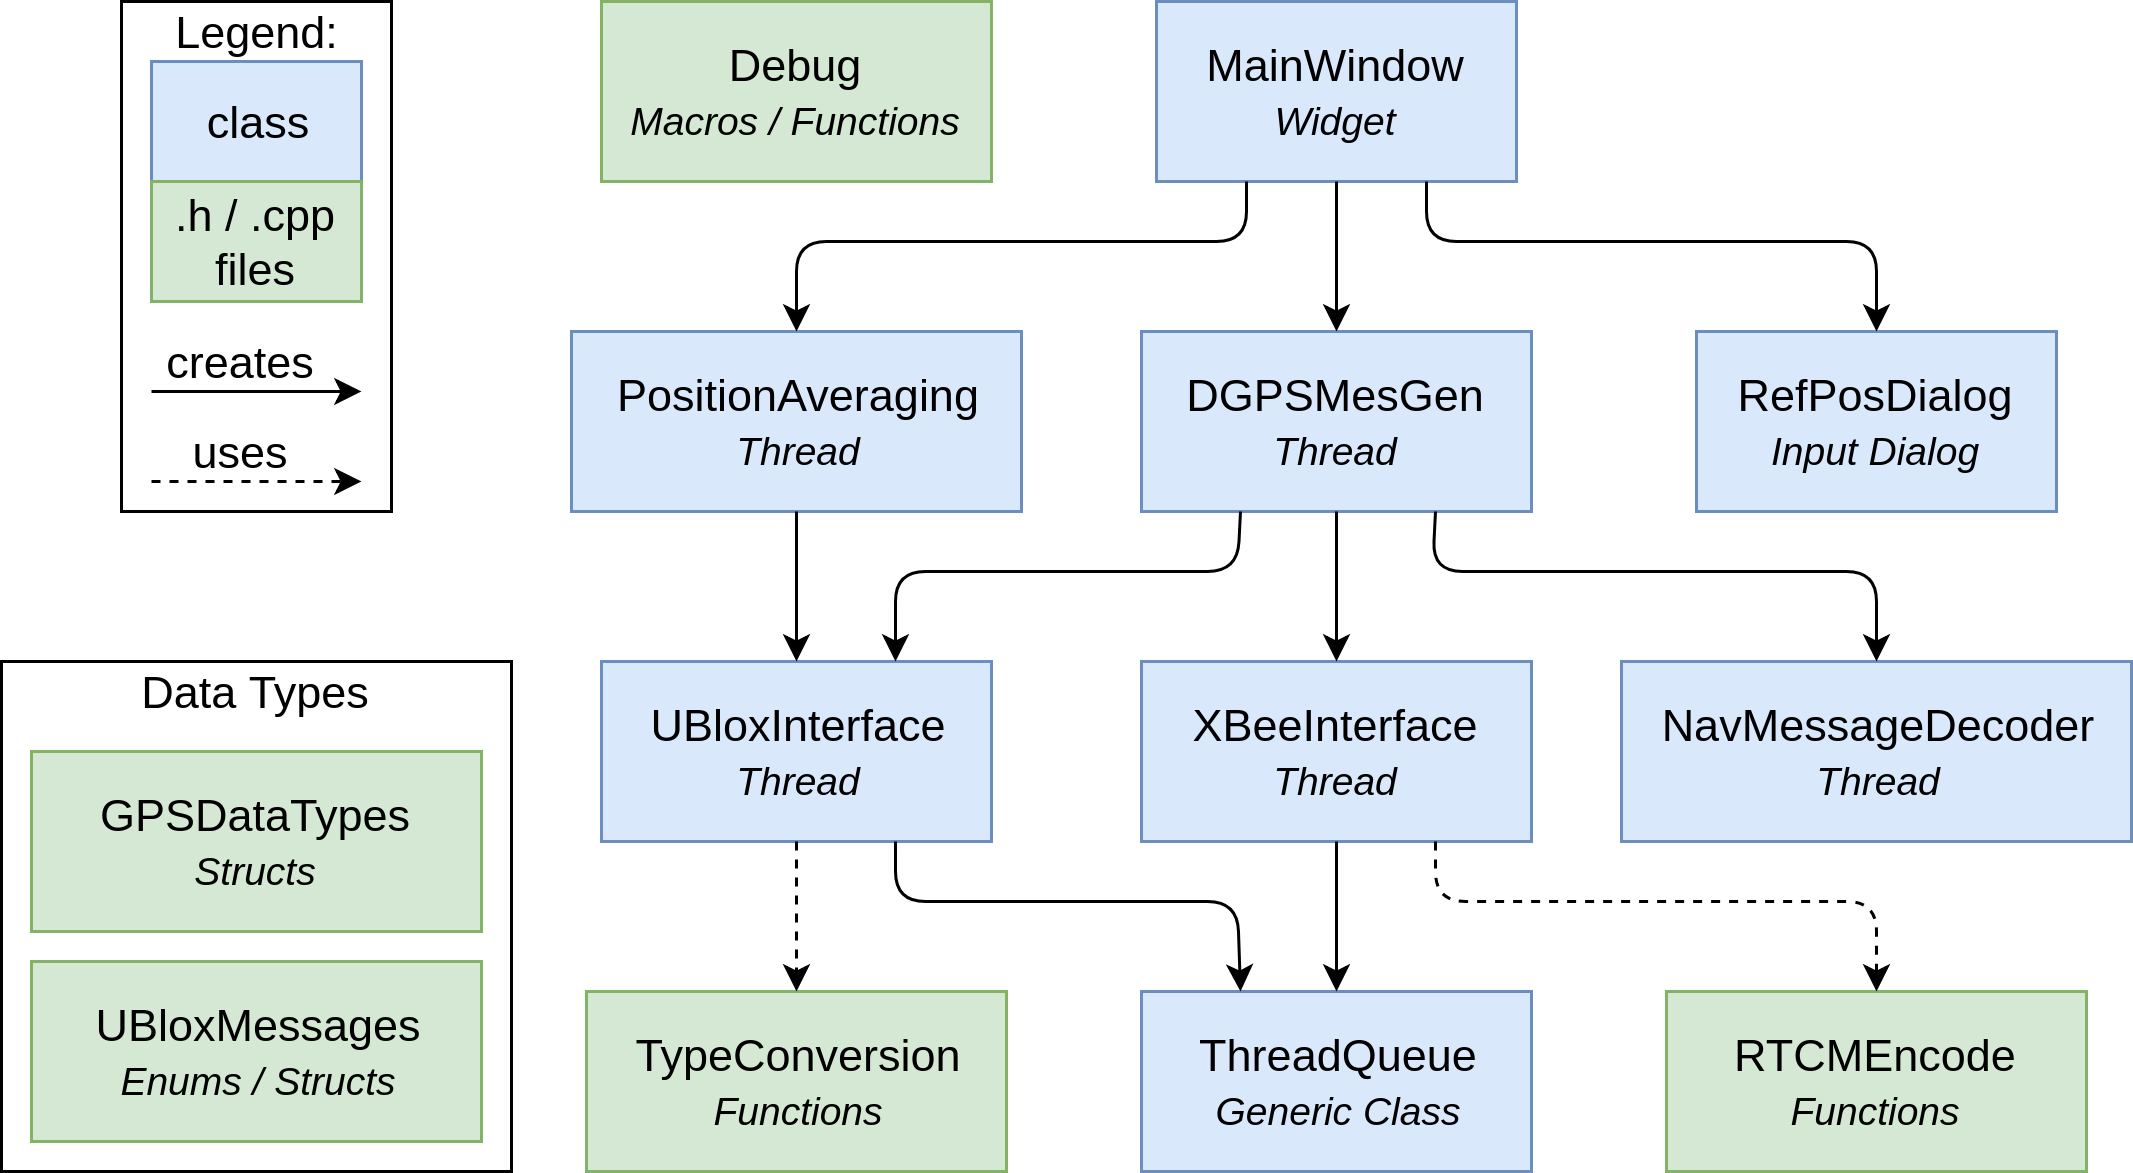
\includegraphics[width=\textwidth]{images/Software_Architecture.png}
\end{frame}

\begin{frame}{Tests}
 \begin{itemize}
  \item Static Accuracy
  \item Mobile Accuracy
  \item Rover / Reference Station Distance
  \item Height Difference \\[15pt]
  \item Antenna Rotation
  \item Correction Message Interruption \\[15pt]
  \item Rocket Launch
 \end{itemize}
\end{frame}


\begin{frame}[standout]
 Questions?
\end{frame}


\end{document}
